\documentclass{book}
\usepackage{graphicx}
\usepackage[utf8]{inputenc}
\usepackage[spanish]{babel}
\usepackage{amsfonts}
\usepackage{bm}

\usepackage{amsmath}
\usepackage{amssymb}

\usepackage{vmargin}

\setpapersize{A4}
\setmargins{2.5cm}       % margen izquierdo
{1.5cm}                        % margen superior
{16.5cm}                      % anchura del texto
{23.42cm}                    % altura del texto
{10pt}                           % altura de los encabezados
{1cm}                           % espacio entre el texto y los encabezados
{0pt}                             % altura del pie de página
{2cm}                           % espacio entre el texto y el pie de página

\title{Introducción al cálculo de variaciones}
\author{Jesús Oroya}



\begin{document}

  
\maketitle
\tableofcontents

\chapter{Introducción al cálculo de variaciones y el control óptimo}
En este documento introduciré brevemente el cálculo de variaciones. Esta es un conocimiento necesario antes de poder entender la formulación de control óptimo y posiblemente el problema \emph{SHE} puede abordarse dentro de este marco. 

El cálculo de variaciones es el análogo a un problema de optimización con variable en $ y\in \mathbb{R}^N $. Com bien sabréis en un problema de optimización deberémos definir claramente la dimensión de la variable de optimización, podría ser un variable escalar, un vector de $\mathbb{R}^2$ o de una dimensión más grande. El cálculo de variaciones aborda un problema donde la variable $y$ tiene dimensión infinita, es decir es una función en sí. 

\section{La geodésica, el camino más corto entre dos puntos }

El problema típico para introducir el cálculo de variaciones es la búsqueda del camino más corto entre dos puntos, la geodésica \footnote{Obviamente el camino más corto que une a dos puntos es la recta, sin embargo por razones pedagógicas utilizaremos este ejemplo}. En general, los libros  suelen introducir este problema pasándo directamente al problema con variables como funciones pero dado que la propuesta es pasar de un problema de optimización en variable discreta a una problema de cálculo variacional empezaremos definiendo el problema de optimización con variable $y \in \mathbb{R}^N$


\subsection{Problema de optimización convencional}

Supongamos que tenemos una secuencia:

\begin{equation}
        \{(x_i,y_i) \}_{0}^{n+1} = \{ (x_0,y_0),(x_1,y_1),\dots,(x_{n+1},y_{n+1})\}
\end{equation}
 
De esta secuencia de puntos conocemos todos los valores de las coordenadas $\{ x_i \}_{i=0}^{n+1} = \{x_0,x_1,\dots,x_{n+1}\}$ además de los valores de las coordenadas  $y_0$ e $y_{n+1}$. 

Entonces, nos podemos preguntar cuál debería ser los valores de las coordenadas $ \{ y_i\}_{i=1}^{n} = \{y_1,\dots,y_n\}$ para que la distancia que define la secuencia $\{x_i,y_i\}_{i=0}^{n+1} $ sea mínima. En la figura (\ref{problema1}) se muestra el problema que proponemos.

\begin{figure}[]
    \centering
    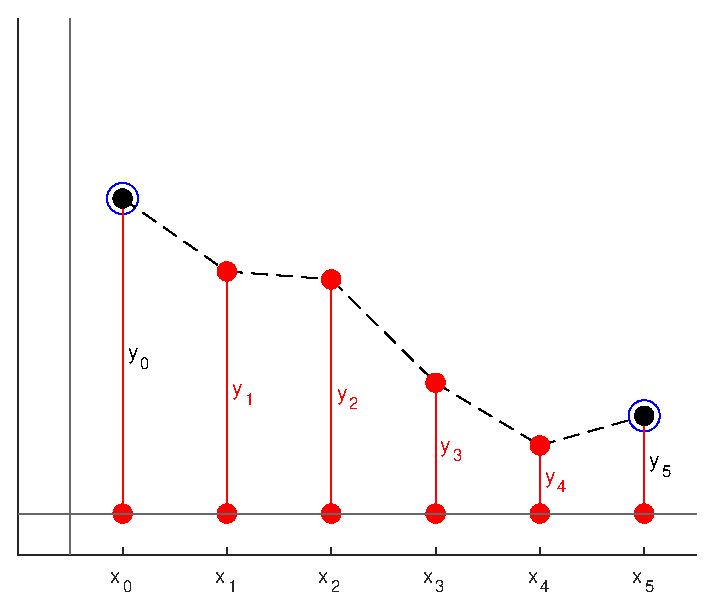
\includegraphics[scale=0.6]{fig/img01.eps}
    \caption{Problema de optimización discreto}
    \label{problema1}
\end{figure}


En un lenguaje más matemático podríamos escribir el problema como la suma de las distancias entre dos puntos consecutivos.
: 

\begin{equation} 
    \min_{\bm{y} \in \mathbb{R}^n} \big[ \sum_{i=1}^{n+1}\sqrt{(x_i - x_{i-1})^2 + (y_i-y_{i-1})^2 }\big]
\end{equation}

Donde $\bm{y} = \{ y_1,y_2,\dots,y_n\}$. Con fines pedagógicos cambiaremos un poco esta expresión para que se pueda comparar fácilmente al problema de cálculo variacional. 

Entonces extraemos $(x_i - x_{i-1})$:


\begin{equation} 
    \min_{\bm{y} \in \mathbb{R}^n} \Bigg[ \sum_{i=1}^{n+1}  (x_i - x_{i-1}) \sqrt{1 + \Bigg( \frac{y_i-y_{i-1}}{x_i - x_{i-1}} \Bigg)^2 }\Bigg]
\end{equation}

Entonces si definimos $\Delta x_i = x_i - x_{i-1}$ y $\Delta y_i = y_i - y_{i-1}  \ | \ \forall i \in \{ 1,\dots,n\}$. Podemos escribir el problema como:

\begin{equation} 
    \min_{\bm{y} \in \mathbb{R}^n} \Bigg[ \sum_{i=1}^{n+1}  \Delta x_i \sqrt{1 + \Bigg( \frac{\Delta y_i}{\Delta x_i } \Bigg)^2 }\Bigg] 
\end{equation}

Para resolver el problema planteado simplemente utilizaremos la condición del gradiente igual a cero  para buscar puntos críticos\footnote{En este problema no existe más puntos críticos que el mínimo por lo que encontrar un punto crítico es igual a encontrar el mínimo y con esto la solución al problema}. 

Llamaremos $d(\bm{y})$ a la función que estamos minimizando, entonces: 

\begin{equation}\label{DiscProb}
    d(\bm{y}) = \sum_{i=1}^{n+1}  \Delta x_i \sqrt{1 + \Bigg( \frac{\Delta y_i}{\Delta x_i } \Bigg)^2 }
\end{equation}

Calculamos la derivada con respecto a $y_i$ de la función $ d(\bm{y})$

\begin{equation}
    \frac{\partial d}{\partial y_i } = 
    \frac{1}{ \big( 1 + (\Delta x_i /\Delta y_i)^2 \big)^{1/2}} -
    \frac{1}{ \big( 1 + (\Delta x_{i-1} /\Delta y_{i-1})^2 \big)^{1/2}} 
\end{equation}

Utilizando la condición necesaria de mínimo $\frac{\partial d }{ \partial y_i} = 0 \ | \ \forall i \in \{ 1, \dots, N \}$, podemos calcular la solución al problema.

\begin{equation}
    \frac{\partial d}{\partial y_i } = 
    \frac{1}{ \big( 1 + (\Delta x_i /\Delta y_i)^2 \big)^{1/2}} -
    \frac{1}{ \big( 1 + (\Delta x_{i-1} /\Delta y_{i-1})^2 \big)^{1/2}} = 0 
\end{equation}
Entonces:
\begin{equation}
    (\Delta y_i /\Delta x_i) = (\Delta y_{i-1} /\Delta x_{i-1}) 
\end{equation}

Por lo tanto la solución al problema es la secuencia que mantenga $(\Delta y_i / \Delta x_i)$ constante. Como notareís este valor el la tangente del angulo formado entre el eje de las abscisa y el vector definido como la unión de dos puntos consecutivos. Es decir, la solución es la secuencia que este alineada. con los puntos $x_0$ y $x_{n+1}$

\subsection{Problema de cálculo de variaciones}

En el problema anterior la variable de optimización vivía en el espacio vectorial $\mathbb{R}^n$. En este caso nos podemos preguntar qué curva que pase por los puntos $(x_0,y_0)$ y $(x_{n+1},y_{n+1})$ es la que tiene menor longitud. La variable en este problema tiene un grado de libertad infinito, es decir en lugar de ser un vector de $\mathbb{R}^n$ es una función $y(x)$ definida en el intervalo $x \in (x_0,x_f)$. Podemos dibujar cualquier función que queramos y deberemos hallar la que minimize la distancia (figura \ref{problema2}). 

Otra pieza fundamental en el cálculo de variaciones es el concepto de funcional. Este es una versión análoga al de función. En el caso de funciones, estas son objetos matemáticas que reciben como entrada un vector  $\bm{y} \in \mathbb{R}^n$ y devuelven un escalar de $d \in \mathbb{R}$. En el caso de los funcionales estos reciben como entrada una función definida en un intervalo y son capaces de devolver un escalar en $\mathbb{R}^n$.

Para hallar la longitud de una curva $y(x)$ que empiece en $(x_0,y_0)$ y termine en $(x_f,y_f)$ tomaremos la expresión (\ref{DiscProb}) tomaremos el límite de cuando $\Delta x_i \rightarrow 0 $


\begin{eqnarray}    
    D[y(x)] = \lim_{\Delta x \rightarrow 0 } d(\bm{y}) = 
    \lim_{\Delta x \rightarrow 0 } \sum_{i=1}^{n+1}  \Delta x_i \sqrt{1 + \Bigg( \frac{\Delta y_i}{\Delta x_i } \Bigg)^2 }
\end{eqnarray}

Utilizando la definición de integral como suma de Riemman:
\begin{eqnarray}      
    \lim_{\Delta x \rightarrow 0 } \sum_{i=1}^{n+1}  \Delta x_i \sqrt{1 + \Bigg( \frac{\Delta y_i}{\Delta x_i } \Bigg)^2 } =
     \int_{x_0}^{x_f}  \sqrt{1 + y'(x) ^2 }  dx 
\end{eqnarray}
Entonces el funcional que nos da la longitud de curva es:
\begin{eqnarray}    
    D[y(x)] =      \int_{x_0}^{x_f}  \sqrt{1 + y'(x) ^2 }  dx 
\end{eqnarray}

Donde $y'(x) = \frac{dy}{dx}$.
\newline


\begin{figure}[h]
    \centering
    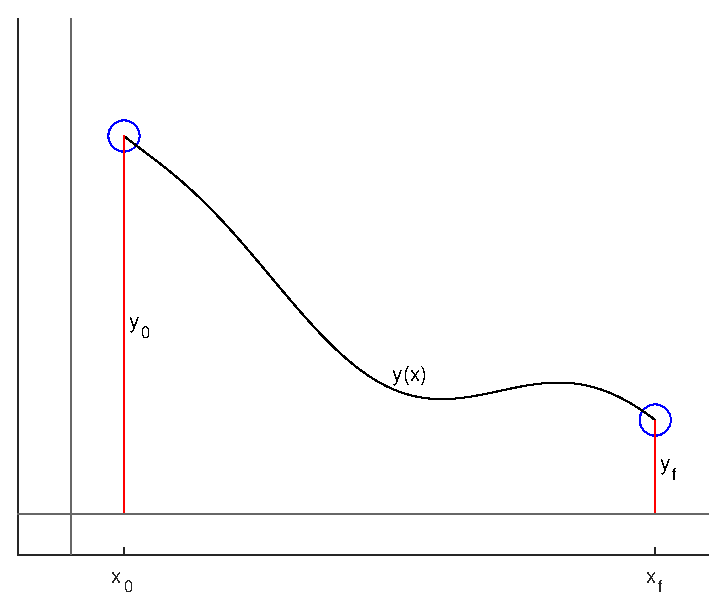
\includegraphics[scale=0.6]{fig/img02}
    \caption{Problema de optimización continuo}
    \label{problema2}
\end{figure}


En calculo de variaciones se le suele llamar lagrangiano $\mathcal{L}(x,y(x),y'(x))$ a la expresión que se encuentra en el interior de la integral. En este caso el lagrangiano sería:

\begin{equation}
    \mathcal{L}(x,y(x),y'(x)) = \sqrt{1 + y'(x) ^2 }
\end{equation}


Al igual que la condición necesaria de mínimo en problemas de optimización convencionales 

\begin{equation}
    \frac{\partial d}{\partial y_i} = 0 \ \ \forall \ i \in \{ 1,\dots,n\}
\end{equation}

En cálculo de variaciones existe una condición necesaria para un mínimo, es es llamada la ecuación de Euler-Lagrange:

\begin{equation}\label{EL}
    \frac{\partial \mathcal{L}}{\partial y(x)} - \frac{d}{dx} \Bigg( \frac{\partial \mathcal{L}}{\partial y'(x)} \Bigg) = 0
\end{equation}

En nuestro caso esta se puede calcular los dos término de la ecuación de Euler-Lagrange fácilmente:

\begin{equation}
    \frac{\partial \mathcal{L}}{\partial y(x)} = \frac{\partial}{\partial y(x)} \Big(\sqrt{1 + y'(x) ^2 } \Big) = 0 
\end{equation}

\begin{equation}
    \frac{\partial \mathcal{L}}{\partial y'(x)}=  \frac{\partial}{\partial y'(x)} \Big(\sqrt{1 + y'(x) ^2 } \Big) = \frac{y'(x)}{\sqrt{1+y'(x)^2}}
\end{equation}

Remplazando estos dos términos en la ecuación (\ref{EL}):

\begin{equation}
    \frac{d}{dx} \Bigg(\frac{y'(x)}{\sqrt{1+y'(x)^2}} \Bigg) = 0
\end{equation}

Es decir:

\begin{equation}
    \Bigg(\frac{y'(x)}{\sqrt{1+y'(x)^2}} \Bigg) = c
\end{equation}

Donde $c$ es una constante. Despejando $y'(x)$ obtenemos:

\begin{equation}
    y'(x) = \frac{c^2}{1-c^2} = m \rightarrow y(x) = mx + b
\end{equation}

Con $m =\frac{c^2}{1-c^2}$ y $b$  constante. Entonces la solución al problema es una recta $y(x) = mx + b$ que pasa por los puntos $(x_0,y_0)$ y $(x_f,y_f)$.

\subsection{Comparación en optimización convencional y cálculo de variaciones}

En la tabla (\ref{tb1}) se muestra analogías entre el cálculo de variaciones y la optimización convencional.

\begin{table}[ht!]
    \begin{tabular}{|c|c|c|}
        \hline
         \textbf{Objeto} & \textbf{Optimización} & \textbf{Cálculo de Variaciones}   \\
         \hline
        Objeto a optimizar & función $d(\bm{y})$ &  funcional $D[y(x)$]\\
        \hline
        Variable de optimización & vector $\bm{y} = \{ y_1,y_2,\dots,y_n\} \in \mathbb{R}^n$ & función $y(x) \ | \ x \in (x_0,x_f)$  \\
        \hline
        Condición de optimalidad & $\frac{\partial d}{\partial y_i} = 0$ & $    \frac{\partial \mathcal{L}}{\partial y(x)} - \frac{d}{dx} \big( \frac{\partial \mathcal{L}}{\partial y'(x)} \big) = 0
        $ \\ 
        \hline
    \end{tabular}
    \caption{Comparación entre la optimización convencional y el cálculo de variaciones} 
    \label{tb1}   
\end{table}


\section{Control Óptimo}

Lllegado a este punto podemos definir el control óptimo como un problema de cálculo variacional donde además tenemos un restricción que deben cumplir las variables en cuestión. De manera general un problema de control óptimo se puede escribir como:

\begin{gather}
    \min_{u \in \mathcal{U} } \Big[ \Psi(y(T)) + \int_0^T L (t,y(t),u(t)) \Big] \\
    \text{sujecto a: } \begin{cases}
        \dot{y} = f(t,y(t),u(t)) \\
        y(0) = y_0
    \end{cases} 
\end{gather}

\subsection{Condiciones de Optimilidad - Principío del mínimo de Pontryagin}

Definimos el Hamiltoniano $H$ como:
\begin{gather}
    H(y(t),u(t),p(t),t) = p^T(t)f(y(t),u(t)) + L(y(t),u(t))
\end{gather}

\begin{gather}
    \begin{cases}
        H(y^*(t),u^*(t),p^*(t),t) \leq  H(y^*(t),u(t),p^*(t),t) \\
        \Psi_T(y(T)) + H(T) = 0 \\
        \dot{p}^T(t) = -H_y(y^*(t),u^*(t),p(t),t) \\
        p^T(T) = \Psi_y(y(T)) 
   \end{cases}
\end{gather}

 
\chapter{Problema SHE como un problema de control óptimo}


Abordaremos el problema de \emph{SHE} de simetría de media onda y de dos niveles. Suponiendo la simetría de media onda de una onda $f(\omega t)$ se puede descomponer en serie de Fourier:

\begin{equation}
    f(\omega t) = \sum_{n=1}^{\infty} \Bigg[ a_n \sin((2n-1)\omega t) + b_n cos((2n-1)\omega t)\Bigg]
\end{equation}

donde:

\begin{equation}
    a_n = \frac{2}{\pi} \int_0^\pi f(\omega t) \sin((2m-1) \omega t) d(\omega t) 
\end{equation}

\begin{equation}
    b_n = \frac{2}{\pi} \int_0^\pi f(\omega t) \cos((2m-1) \omega t) d(\omega t) 
\end{equation}

Para simplificar harémos el cambio de variable $\tau = \omega t$. Entonces las expresiones anteriores se pueden escribir de la siguiente forma:

\begin{equation}
    f(\tau) = \sum_{n=1}^{\infty} \Bigg[ a_n \sin((2n-1)\tau) + b_n cos((2n-1)\tau)\Bigg]
\end{equation}

\begin{equation}\label{an}
    a_n = \frac{2}{\pi} \int_0^\pi f(\tau) \sin((2m-1) \tau) d\tau 
\end{equation}
\begin{equation}\label{bn}
    b_n = \frac{2}{\pi} \int_0^\pi f(\tau) \cos((2m-1) \tau) d\tau 
\end{equation}

Deberemos notar que las expresiones (\ref{an}) y (\ref{bn}) pueden ser escritas en forma de ecuación diferencial:

\begin{gather}
    a_n = \frac{2}{\pi} \int_0^\pi f(\tau) \sin((2m-1) \tau) d\tau  \  \Rightarrow \ \frac{d \alpha_n}{d\tau} = \frac{2}{\pi}f(\tau) \sin((2m-1)\tau) \ | \ \alpha_n(0) = 0\\ 
    b_n = \frac{2}{\pi} \int_0^\pi f(\tau) \cos((2m-1) \tau) d\tau  \  \Rightarrow \ \frac{d \beta_n}{d\tau} = \frac{2}{\pi}f(\tau) \cos((2m-1)\tau) \ | \ \beta_n(0) = 0
\end{gather}

Entonces dado una función $f(\tau)$ podemos obtener los coeficiente de Fourier $a_n$ y $b_n$ resolviendo el siguiente sistema de ecuaciones diferenciales hasta tiempo $\tau=\pi$.

\begin{gather}
    \frac{d \alpha_n}{d\tau} = \frac{2}{\pi}f(\tau) \sin((2m-1)\tau) \ | \ \alpha_n(0) = 0 \\
    \frac{d \beta_n}{d\tau} = \frac{2}{\pi}f(\tau) \cos((2m-1)\tau) \ | \ \beta_n(0) = 0
\end{gather}

\section{Problema de control óptimo para SHE}
De esta forma si tenemos un vector de objetivo $\bm{a}_T = [a_1^T,a_2^T,\dots,a_{M}^T] \in \mathbb{R}^M$ y  $\bm{b}_T = [b_1^T,b_2^T,\dots,b_{M}^T] \in \mathbb{R}^M$, donde $M$ es el número de armónicos impares de interés, podemos plantear el siguiente problema de control óptimo:

\begin{gather}
    \min_{f(\tau) \in \mathcal{F}} \big[  || \bm{\alpha}(T) - \bm{a}_T ||^2  + || \bm{\beta}(T) - \bm{b}_T ||^2 \big] \\
    \text{sujeto a: }
    \begin{cases}
        \frac{d \alpha_n}{d\tau} = \frac{2}{\pi}  f(\tau) \sin[(2m-1) \tau ] \ \ \ | \ \ \ a(0) = 0   \\
        \frac{d \beta_n}{d\tau}  = \frac{2}{\pi}  f(\tau) \cos[(2m-1) \tau ] \ \ \ | \ \ \ b(0) = 0   \\
    \end{cases}
    \forall n \in \{ 1, \dots,M\}  \\ 
    \text{sujeto a: } f_{min} < f(\tau) < f_{max} \ | \ \forall \ \tau \in (0,\pi)  
\end{gather}

Con tiempo final $T = \pi$


\section{Condiciones de optimalidad  para el problema de control óptimo para SHE}


Siguiendo el principio de mínimo de Pontryagin construiremos el Hamiltoniano:

\begin{gather}
    H = \sum_{m=1}^M \Bigg[ p_\alpha^m \Bigg(\frac{2}{\pi} f(\tau) \sin((2m-1)\tau)\Bigg) + p_\beta^m \Bigg(\frac{2}{\pi} f(\tau) \cos((2m-1)\tau)\Bigg) \Bigg] \\
    H = \frac{2}{\pi} f(\tau)\sum_{m=1}^M \Bigg[  p_\alpha^m   \sin \big[(2m-1)\tau)\big] 
                                                + p_\beta^m   \cos \big[ (2m-1)\tau)\big] \Bigg]
\end{gather}
 
La ecuación de adjunto se puede calcular de la siguiente manera:

\begin{gather}
    \frac{d p_\alpha^m}{d \tau} = \frac{\partial H }{\partial \alpha_m} = 0 \ \ \text{y} \ \    \frac{d p_\beta^m}{d \tau} = \frac{\partial H }{\partial \beta_m} = 0  
\end{gather}

Es decir la componente $p_\alpha^n$ y $p_\beta^n$ son constantes.
\newline

Si llamamos $\Psi(\bm{\alpha},\bm{\beta})$ a:

\begin{gather}
    \Psi(\bm{\alpha},\bm{\beta}) = \big[  || \bm{\alpha}(T) - \bm{a}_T ||^2  + || \bm{\beta}(T) - \bm{b}_T ||^2 \big]
\end{gather}
Utilizando la condición final del adjunto:

\begin{gather}
    p_\alpha^m(T) = \frac{d\Psi}{d\alpha_m} = 2(\bm{\alpha_m(T) - \bm{a}^T_n})\\
    p_\beta^m(T) = \frac{d\Psi}{d\beta_m} = 2(\bm{\beta_m(T) - \bm{b}^T_n})
\end{gather}


Si llamamos $G(\tau,\bm{p}_\alpha,\bm{p}_\beta)$ a:

\begin{gather}
    G(\tau,\bm{p}_\alpha,\bm{p}_\beta) =  \frac{2}{\pi}\sum_{m=1}^M \Bigg[  p_\alpha^m   \sin \big[(2m-1)\tau)\big] 
    + p_\beta^m   \cos \big[ (2m-1)\tau)\big] \Bigg]
\end{gather}

Entonces el Hamiltoniano se puede escribir como: 

\begin{gather}
    H = G(\tau,\bm{p}_\alpha,\bm{p}_\beta) f(\tau)
\end{gather}

Aplicando el principio del mínimo de Pontryagin podemo hallar la forma de $f^*$ 

\begin{gather}
    \min_{f \in \mathcal{F}} H \rightarrow f^* = \begin{cases}
        f_{min} \ \  \text{si} \ \ G(\tau,\bm{p}_\alpha,\bm{p}_\beta) > 0  \\
        f_{max} \ \ \text{si}  \ \ G(\tau,\bm{p}_\alpha,\bm{p}_\beta) < 0  
    \end{cases}
\end{gather}

Obtenemos un control \emph{Bang-Bang}, es decir una función que toma solo dos valores (\ref{figbang})



\begin{figure}[]
    \centering
    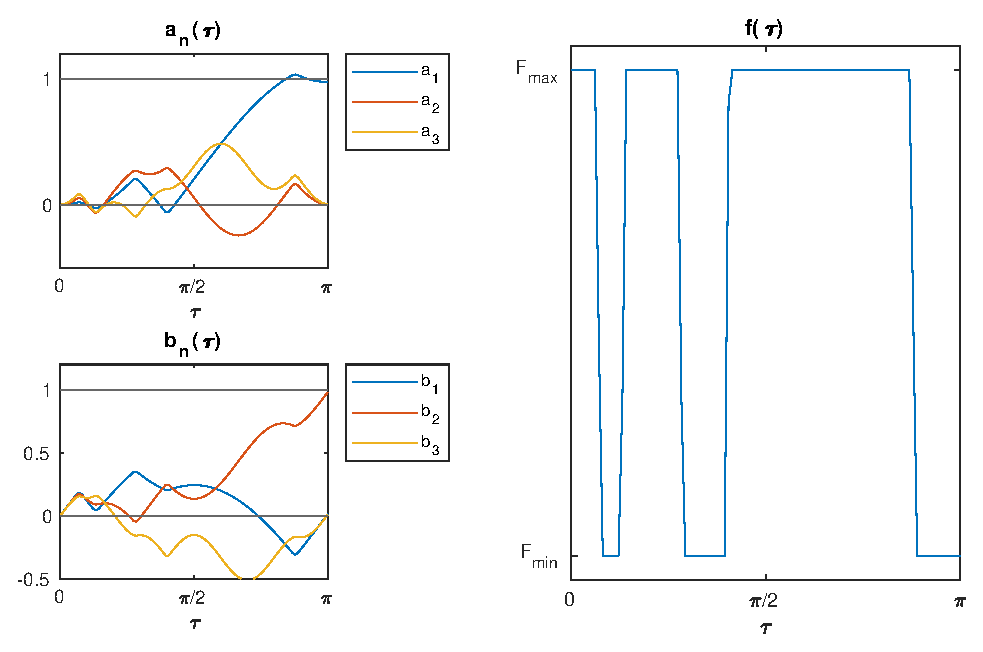
\includegraphics[scale=0.7]{fig/img03.eps}
    \caption{Solución numérico del problema de control óptimo. $a_T = [1 \ 0 \ 0 \ 0]^T$ y 
    $b_T = [1 \ 0 \ 1 \ 0]^T$}
    \label{figbang}
\end{figure}


  

\end{document}